\graphicspath{{./figures/}}
\title{}
\date{}
\begin{document}
\begin{frame}
    \titlepage
\end{frame}

\begin{frame}{last time}
    \begin{itemize}
    \item dynamic linking
        \begin{itemize}
        \item global offset table
        \item stubs
        \item lazy binding
        \end{itemize}
    \item viruses calling standard library
    \item integrity checking files
        \begin{itemize}
        \item tripwire: did it change?
        \item application signing
        \item limitations
            \begin{itemize}
            \item malware in scripts
            \item malicious software in ``data'' files
            \item downloaded software people want to run
            \end{itemize}
        \end{itemize}
    \item searching for patterns
        \begin{itemize}
        \item regular expression matching
        \end{itemize}
    \end{itemize}
\end{frame}

\usetikzlibrary{arrows.meta,calc,fit,matrix,positioning,shapes.callouts}

\subsection{flex state machines}
\usetikzlibrary{arrows.meta,automata,positioning}

\begin{frame}[fragile,label=flexSM]{flex: state machines}
\lstset{
        style=small,
        language={},
        moredelim={**[is][\btHL<2|handout:0>]{@hi2@}{@endhi@}},
        }
\begin{lstlisting}
foo     {...}
.       {...}
\n      {...}
\end{lstlisting}
\begin{tikzpicture}
\begin{scope}[every node/.style={font=\tt,thick}]
\node[initial,state,font=\normalfont\it] (start) {};
\node[state,right=1cm of start] (f) {f};
\node[state,right=1cm of f] (fo) {fo};
\node[state,right=1cm of fo,accepting] (foo) {foo};
\node[state,below right=2cm of start,accepting] (dot) {.};
\node[state,below=1.5cm of start,accepting] (newline) {\textbackslash{}n};
\end{scope}
\path[-Latex,thick] (start) edge node[above] {\tt f} (f)
                    (f) edge node[above] {\tt o} (fo)
                    (fo) edge node[above] {\tt o} (foo)
                    (start) edge node[sloped,above] {other} (dot)
                    (start) edge node[left] {\textbackslash{}n} (newline);
\begin{visibleenv}<2>
    \path[-Latex,blue,dashed] (f) edge node[right] {(back 1)} (dot);
    \path[-Latex,blue,dashed] (fo) edge[out=-45,in=-30] node[midway, sloped, below] {(back 2)} (dot);
\end{visibleenv}
\end{tikzpicture}
\end{frame}

\begin{frame}[fragile,label=stateMachineMatch]{state machine matching}
\begin{tikzpicture}
\node(matchString) {\large \tt \sout<3->{\myemph<2>{a}}\sout<4->{b}\sout<7->{\myemph<5-6>{f}\myemph<6>{oo}}\myemph<7-8>{f}\myemph<7>{\sout<8>{o}}abffoo};

\begin{scope}[every node/.style={font=\tt,thick}]
\node[initial, state,below=1cm of matchString,font=\normalfont\it,
      alt=<2>{red}{}] (start) {};
\node[state,right=1cm of start,alt={<5,7>{red}{}}] (f) {f};
\node[state,right=1cm of f,alt={<6,7>{red}{}}] (fo) {fo};
\node[state,right=1cm of fo,accepting,alt={<6>{red}{}}] (foo) {foo};
\node[state,below right=2cm of start,accepting,alt={<3,8>{red}{}}] (dot) {.};
\node[state,below=1.5cm of start,accepting] (newline) {\textbackslash{}n};
\end{scope}
\path[-Latex,thick] (start) edge[alt=<5-7>{red}{}] node[above] {\tt f} (f)
                    (f) edge node[above,alt=<6>{red}{}] {\tt o} (fo)
                    (fo) edge node[above,alt=<6>{red}{}] {\tt o} (foo)
                    (start) edge node[sloped,above,alt=<3>{red}{}] {other} (dot)
                    (start) edge node[left] {\textbackslash{}n} (newline);
\path[-Latex,blue,dashed] (f) edge node[right] {(back 1)} (dot);
\path[-Latex,blue,dashed,alt=<8>{red,thick}{}] (fo) edge[out=-45,in=-30] node[midway, sloped, below] {(back 2)} (dot);
\end{tikzpicture}
\end{frame}





    % FIXME: more complex state machine


\begin{frame}{why this?}
    \begin{itemize}
    \item one pass matching (except for some backtracking)
        \begin{itemize}
        \item can make state machine bigger to avoid some backtracking
        \end{itemize}
    \item basically speed of file I/O
    \item handles multiple patterns well
    \item flexible for ``special cases''
    \vspace{.5cm}
    \item<2> real anti-virus: probably custom pattern ``engine''
    \end{itemize}
\end{frame}




\subsection{backtracking problems?}
\input{../heur-detect/flex-opt-btp}


\usetikzlibrary{arrows.meta,automata,positioning}

\begin{frame}[fragile,label=noBt]{avoiding backtracking?}
\lstset{
        style=small,
        language={},
        moredelim={**[is][\btHL<2|handout:0>]{@hi2@}{@endhi@}},
        }
\begin{lstlisting}
fox  {...}
foo  {...}
off  {...}
.|\n {/* do nothing */}
\end{lstlisting}
\begin{tikzpicture}
\begin{scope}[every node/.style={font=\tt,thick}]
\node[initial, state,below=2cm,font=\normalfont\it] (start) {};
\node[state,above right=1cm of start] (f) {f};
\node[state,right=1cm of f] (fo) {fo};
\node[state,above right=1cm of fo,accepting] (fox) {fox};
\node[state,right=1cm of fo,accepting] (foo) {foo};
\node[state,below right=1cm of start] (o) {o};
\node[state,right=1cm of o] (of) {of};
\node[state,right=1cm of of,accepting] (off) {off};
\end{scope}
\path[-Latex,thick]
                    (start) edge[loop below] node[below] {other} (start);
\path[-Latex,thick]
                    (start) edge node[above] {\tt f} (f)
                    (f) edge node[above] {\tt o} (fo)
                    (fo) edge node[above] {\tt o} (foo)
                    (fo) edge node[above] {\tt x} (fox)
                    (start) edge node[above] {\tt o} (o)
                    (o) edge node[above] {\tt f} (of)
                    (of) edge node[above] {\tt f} (off);
\path[red,-Latex,thick] (f) edge node[right,align=left] {\tt o} (o);
\path[red,-Latex,thick] (of) edge node[right,align=left] {\tt o} (f);
\path[red,-Latex,thick] (fo) edge node[right,align=left] {\tt f} (of);
\node[overlay] at (fox.north west) {not shown: extra edges to start};
\end{tikzpicture}
\end{frame}



\subsection{flex: Vienna example}

\begin{frame}[fragile,label=ViennaPat1]{Vienna patterns (1)}
\lstset{
        style=small,
        language={},
        moredelim={**[is][\btHL<2|handout:0>]{@hi2@}{@endhi@}},
        escapechar=`,
        }
\begin{itemize}
\item simple Vienna patterns:
\end{itemize}
\begin{lstlisting}
/* bytes of fixed part of Vienna sample */
\xFC\x89\xD6\x83\xC6\x81\xc7\x00\x01\x83`\textit{(etc)}` {
        printf("found Vienna code\n");
    }
\end{lstlisting}
\end{frame}


\begin{frame}[fragile,label=ViennaPat2]{Vienna patterns (2)}
\lstset{
        style=small,
        language={},
        moredelim={**[is][\btHL<2|handout:0>]{@hi2@}{@endhi@}},
        escapechar=`,
        }
\begin{itemize}
\item simple Vienna patterns:
\end{itemize}
\begin{lstlisting}
/* Vienna sample with wildcards for
   changing bytes: */
/* push %CX; mov ???, %dx; cld; ... */
\x51\xBA@hi2@(.|\n)(.|\n)@endhi@\xFC\x89`\textit{(etc)}` {
        printf("found Vienna code w/placeholder\n");
    }
/* mov $0x100, %di; push %di; xor %di, %di; ret */
\xBF\x00\x01\x57\x31\xFF\xC3 {
        printf("found Vienna return code\n");
    }
\end{lstlisting}
\end{frame}




\subsection{why the flexibility?}
\begin{frame}{regular expressions are flexible}
    \begin{itemize}
    \item for Vienna: lots of flex features we didn't need
        \begin{itemize}
        \item things being repeated variable number of times
        \item one of list of possible characters (bytes)
        \item \ldots
        \end{itemize}
    \vspace{.5cm}
    \item but viruses try to make pattern matching hard
    \item good to think about what we can easily match
    \end{itemize}
\end{frame}

% FIXME: exercise
\subsection{exercise: what's easy/hard for patterns}

    % most/least suitable to pattern matching
        % Vienna inserting random number of nops every 8 instructions of virus code
        % Vienna, but replacing code at a random offset in the executable
        % virus code, but with registers for temporaries used chosen at random
        % virus code, but most of the code split into cavities and a "loader" that reforms it placed at a fixed location

\begin{frame}{hard for patterns?}
    \begin{itemize}
    \item malware makes modificates to evade pattern matching
    \item exercise: suppose we have a pattern for a Vienna-like virus, and a new version makes the following
        change. Which of the following is going to be easiest/hardest to change the pattern for?
        \begin{itemize}
        \item A. inserting random number of nops every 8 non-nop instructions of virus code
        \item B. replacing code at random offset in executable instead of appending
        \item C. registers used for temporaries in virus code chosen at random each time the virus copies itself
        \item D. instead of appending all the virus code, virus code now split between cavities with a "loader" appended (the "loader" reforms code from the cavities and jumps to them)
        \end{itemize}
    \end{itemize}
\end{frame}


\section{making scanners more efficient}
\usetikzlibrary{matrix,shapes.misc}

\begin{frame}<1>[label=effScanners]{making scanners efficient}
    \begin{itemize}
    \item \myemph<2>{lots of viruses!}
        \begin{itemize}
        \item huge number of states, tables
        \item copies of every piece of malware pretty large
        \end{itemize}
    \item \myemph<3>{reading files is slow!}
    \end{itemize}
\end{frame}



\subsection{fixed strings}
\againframe<2>{effScanners}
\input{../heur-detect/fixed-strings}

\subsection{selective scanning}
\againframe<3>{effScanners}

\begin{frame}{the I/O problem}
    \begin{itemize}
    \item scanning still requires reading the whole file
    \item can we do better?
    \end{itemize}
\end{frame}

\begin{frame}{selective scanning}
    \begin{itemize}
    \item check entry point and end only
        \begin{itemize}
        \item a lot less I/O, maybe
        \end{itemize}
    \item check known offsets from entry point
    \item heuristic: is entry point close to end of file?
    \end{itemize}
\end{frame}



\section{example: ClamAV}
    % FIXME: show example patterns and more
\input{../heur-detect/example-clam-av}

\section{new malware detection?}

\begin{frame}{playing cat}
    \begin{itemize}
    \item harder to fool ways of detecting malware?
    \item goal: small changes to malware preserve detection
    \item ideal: detect \myemph{new} malware
    \end{itemize}
\end{frame}

\begin{frame}<1>[label=detectNew]{detecting new malware}
    \begin{itemize}
    \item \myemph<2>{look for anomalies}
        \begin{itemize}
        \item patterns of code that real executables ``won't'' have
        \end{itemize}
    \item \myemph<3>{identify bad behavior}
    \end{itemize}
\end{frame}




\section{heuristics based on executable/library regularity}

\begin{frame}{viruses and executable formats}
\begin{tikzpicture}
\tikzset{
    mybox/.style={draw,rectangle,minimum width=10cm,fill=white},
}
\node[mybox] (header) {
    \textbf{header}: machine type, file type, etc.
};
\node[mybox,below=0mm of header,align=center] (pHeader) {
    \textbf{program header}: ``\myemph{segments}'' to load \\
        (also, some other information) \\
    \only<2-3>{\myemph{\textbf{length edited by virus}}}
    \only<4-6>{\myemph{\textbf{new segment added by virus}}}
};
\node[mybox,below=0mm of pHeader,align=center] (seg1) {
    \textbf{segment 1 data}
};
\node[mybox,below=0mm of seg1,align=center] (seg2) {
    \textbf{segment 2 data} \\
    \only<2-3>{\myemph{\textbf{virus code + new entry point?}}}
};
\node[mybox,visible on=<4-6>,below=0mm of seg2,align=center] (seg3) {
    \myemph{\textbf{segment 3 data --- virus segment}}
};
\coordinate (annotate) at ([yshift=-1.5cm]seg2.south);
\tikzset{
    annoBox/.style={draw=red,thick,at=(annotate),font=\small,align=center},
}
\begin{visibleenv}<3,5>
    \node[annoBox] {heuristic 1: is entry point in last segment? \\ (segment usually not code)};
\end{visibleenv}
\begin{visibleenv}<6>
    \node[annoBox] {heuristic 2: did virus mess up header? \\ (e.g. do sizes used by linker but not loader disagree)
                \\ section names disagree with usage?};
\end{visibleenv}
\end{tikzpicture}
\end{frame}

\begin{frame}{defeating entry point checking}
    \begin{itemize}
    \item \myemph<2>{insert jump in normal code section, set as entry-point}
    \item add code to first section instead (perhaps insert new section at beginning)
    \end{itemize}
\begin{tikzpicture}
\tikzset{
    annoBox/.style={draw=red,thick,align=center},
}
    \begin{visibleenv}<2>
    \node[annoBox] {
        ``dynamic'' heuristic: run code in VM, see if switches sections
    };
    \end{visibleenv}
\end{tikzpicture}
\end{frame}

\begin{frame}{heuristics: library calls}
    \begin{itemize}
    \item dynamic linking --- functions called \myemph{by name}
    \item how do viruses add to dynamic linking tables?
        \begin{itemize}
        \item often don't! --- instead dynamically look-up functions
        \item if do --- could mess that up/lots of code
        \end{itemize}
    \end{itemize}

    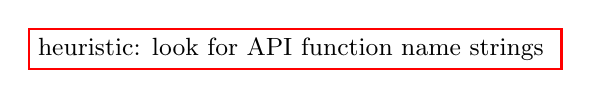
\begin{tikzpicture}
\tikzset{
    annoBox/.style={draw=red,thick,font=\small,align=center},
}
    \node[annoBox] {
        heuristic: look for API function name strings
    };
    \end{tikzpicture}
\end{frame}

\begin{frame}{evading library call checking}
    \begin{itemize}
    \item modify dynamic linking tables
        \begin{itemize}
        \item probably tricky to add new entry
        \end{itemize}
    \item reimplement library call manually
        \begin{itemize}
        \item Windows system calls not well documented, change
        \end{itemize}
    \item \myemph<2>{hide names}
    \end{itemize}
\end{frame}

\begin{frame}{hiding library call names}
    \begin{itemize}
    \item common approach: store \myemph{hash of name}
    \item runtime: read library, scan list of functions for name
    \vspace{.5cm}
    \item bonus: makes analysis harder
    \end{itemize}
\end{frame}




\section{behavior based detection}
\begin{frame}{behavior-based detection}
    \begin{itemize}
    \item things malware does that other programs don't?
    \vspace{.5cm}
    \item<2-> modify system files
    \item<2-> modifying existing executables
    \item<2-> open network connections to lots of random places 
    \item<2-> \ldots
    \vspace{.5cm}
    \item basic idea: run in virtual machine; and/or monitor all programs
    \end{itemize}
\end{frame}


\subsection{instrumenting programs}
\begin{frame}<1>[label=hookingList]{hooking}
    \begin{itemize}
    \item hooking --- getting a `hook' to run on (OS) operations
        \begin{itemize}
        \item e.g. creating new files
        \item e.g. modifying executable files
        \end{itemize}
    \item ideal mechanism: \myemph<2>{OS support}
    \item less ideal mechanism: \myemph<3>{change library loading}
        \begin{itemize}
        \item e.g. replace `open', `fopen', etc. in libraries
        \end{itemize}
    \item less ideal mechanism: \myemph<4>{replace OS exception} (system call) handlers
        \begin{itemize}
        \item very OS version dependent
        \end{itemize} 
    \item less ideal mechanism: \myemph<5>{debugger support}
    \end{itemize}
\end{frame}

\againframe<2>{hookingList}

\begin{frame}
\includegraphics[height=0.9\textheight]{../heur-detect/filter-driver} 
\end{frame}

\begin{frame}{Linux hooking}
\begin{itemize}
\item several possible mechanisms
\item tracepoints, kprobes
    \begin{itemize}
    \item cause hooking functions to run when kernel functions called or return
    \item hooker function can arrange for logging or other action
    \end{itemize}
\item seccomp BPF
    \begin{itemize}
    \item allow hooker to write `program' to examine system calls of selected processes
    \item can deny/change/log those system calls
    \end{itemize}
\end{itemize}
\end{frame}

\begin{frame}{aside Linux eBPF}
    \begin{itemize}
    \item eBPF = extended Berkeley Packet Filters
    \item little programming language originally intended for network filtering
    \item 
    \end{itemize}
\end{frame}

\againframe<3>{hookingList}

\begin{frame}{changing library loading}
\begin{itemize}
    \item e.g. install new library --- or edit loader, but \ldots
    \vspace{.5cm}
    \item not everything uses library functions
    \item what if your wrapper doesn't work exactly the same?
\end{itemize}
\end{frame}

\againframe<4>{hookingList}

\begin{frame}{changing exception call handlers (1)}
    \begin{itemize}
    \item OS data structure tells hardware where program requests go
    \item simpliest mechanism: edit that data structure
       \begin{itemize}
       \item and save a copy of what was there before
       \end{itemize}
    \item point to your code
        \begin{itemize}
        \item and call what was there before after behavior check
        \end{itemize}
    \end{itemize}
\end{frame}



\section{AI heuristic case study: DREBIN}

\begin{frame}{heuristics example: DREBIN paper}
    \begin{itemize}
    \item {\small from 2014 research paper on Android malware: Arp et al, ``DREBIN: Effective and Explainable Detection of Android Malware in Your Pocket''}
    \item primary contribution of paper: big dataset of malware
    \item but tried to detect malware, too\ldots
    \item features from applications (\myemph{without running}):
        \begin{itemize}
        \item hardware requirements
        \item requested permissions
        \item whether it runs in background, with pushed notifications, etc.
        \item what API calls it uses
        \item network addresses
        \end{itemize}
    \item detect \myemph{dynamic code generation} explicitly
    \item statistics (i.e. machine learning) to determine score
    \end{itemize}
\end{frame}

\begin{frame}{heuristics example: DREBIN paper}
    \begin{itemize}
    \item advantage: Android uses Dalvik bytecode (Java-like)
        \begin{itemize}
        \item high-level ``machine code''
        \item much easier/more useful to analyze
        \end{itemize}
    \item accuracy?
        \begin{itemize}
        \item tested on 131k apps, $94$\% of malware, $1$\% false positives
        \item versus best commercial: $96$\%, $<0.3$\% false positives
            \begin{itemize}
            \item (probably has explicit patterns for many known malware samples)
            \end{itemize}
        \end{itemize}
    \item \ldots but
        \begin{itemize}
        \item statistics: training set needs to be typical of malware
        \item cat-and-mouse: what would attackers do in response?
        \end{itemize}
    \end{itemize}
\end{frame}


\subsection{machine learning and adversaries}
\begin{frame}{machine learning and adversaries}
    \begin{itemize}
    \item I don't like most ML-based approaches to malware detection
    \vspace{.5cm}
    \item problem: most machine learning not designed to deal with adversaries
    \item attack: find factors used to ID benign programs
        \begin{itemize}
        \item do all of them as much as possible
        \item inquiry: what might they be in DREBIN case?
        \end{itemize}
    \item attack: provide many malware samples with benign weird behavior
        \begin{itemize}
        \item machine learning uses weird behavior to identify malware
        \item may lower effectiveness on `normal' malware
        \end{itemize}
    \end{itemize}
\end{frame}


\section{anti-anti-virus}

\begin{frame}{anti-anti-virus}
    \begin{itemize}
    \item defeating signatures:
    \vspace{.5cm}
    \item avoid things compilers/linkers never do
    \item make analysis harder
        \begin{itemize}
        \item takes longer to produce signatures
        \item takes longer to produce ``repair'' program
        \item may evade attempts to automate analysis
        \end{itemize}
    \item make changing viruses
        \begin{itemize}
        \item make any one signature less effective
        \end{itemize}
    \end{itemize}
\end{frame}





\begin{frame}{some terms}
    \begin{itemize}
    \item \myemph{armored} viruses
        \begin{itemize}
        \item viruses designed to make analysis harder
        \end{itemize}
    \item \myemph{metamorphic}/\myemph{polymorphic}/\myemph{oligomorphic} viruses
        \begin{itemize}
        \item viruses that change their code each time
        \item different terms --- different types of changes (later)
        \end{itemize}
    \end{itemize}
\end{frame}


\section{other obfuscation}
\subsection{why obfuscation, generally}
\begin{frame}{obfuscation, generally}
    \begin{itemize}
    \item malware often \textit{obfuscates} (obscures) its code
    \item several reasons for this
        \begin{itemize}
        \item prevent their from being signatures
        \item make analysis more difficult
        \item prevent others from modifying+copying
        \end{itemize}
    \vspace{.5cm}
    \item note: many of these technique sometimes employed by commercial software
        \begin{itemize}
        \item intended to prevent copying/reverse-engineering
        \end{itemize}
    \end{itemize}
\end{frame}


\section{Tigress and its transformations}
\begin{frame}{Tigress as example of obfuscation}
    \begin{itemize}
    \item Tigress --- researcher developer obfuscation tool
    \item \texttt{https://tigress.wtf}
    \item includes many \textit{transformations} typical of real-world obfuscation
        \begin{itemize}
        \item we'll talk about the ideas behind many of them
        \end{itemize}
    \vspace{.5cm}
    \item future assignment: modify code obfuscated with Tigress
    \end{itemize}
\end{frame}
\begin{frame}{example Tigress transformations}
    \begin{itemize}
    \item we'll look at some simple ones Tigress provides
    \item I'm showing you the pattern, \\ not the actual code Tigress generates
    \end{itemize}
\end{frame}

\begin{frame}[fragile,label=TigressMerge]{Tigress: provided transform: Merge}
\begin{lstlisting}[language=C++,style=smaller]
void foo(int a) { code for foo }
void bar(int a) { code for bar }

... foo(x) + bar(y) ...
\end{lstlisting}
\hrule
\begin{lstlisting}
void foo_bar(int s, int a) {
    if (s == 0) {
        code for foo
    } else {
        code for bar
    }
}

... foo_bar(0, x) + foo_bar(1, y) ...
\end{lstlisting}
\end{frame}

\begin{frame}[fragile,label=TigressSplit]{Tigress: provided transform: Split}
\begin{lstlisting}[language=C++,style=smaller]
void foo(int a, int b) {
    int x = ...;
    code for foo part 1
    code for foo part 2
}
\end{lstlisting}
\hrule
\begin{lstlisting}[language=C++,style=smaller]
void foo1(int *a, int *b, int *x) {
    code for foo part 1
}
void foo2(int *a, int *b, int *x) {
    code for foo part 2
}
void foo(int a, int b) {
    int x;
    foo1(&a,&b,&x); foo2(&a,&b,&x);
}
\end{lstlisting}
\end{frame}

\begin{frame}[fragile,label=TigressFlatten]{Tigress: example transform: Flatten}
\begin{lstlisting}[language=C++,style=smaller]
void foo() {
    A;
    if (X) {
        B;
    } else {
        C;
    }
    D;
}
\end{lstlisting}
\hrule
\begin{lstlisting}[language=C++,style=smaller]
void foo() {
    int s = 0;
    for (;;) {
        switch(s) {
        case 0: A; s = X ? 1 : 2; break;
        case 1: B; s = 3; break;
        case 2: C; s = 3; break;
        case 3: D; return;
        }
    }
}
\end{lstlisting}
\end{frame}

\begin{frame}{transformations so far?}
    \begin{itemize}
    \item all can be combined!
    \item annoying for analysis
    \item hard to do without unobfuscated code
        \begin{itemize}
        \item can't easily be redone/changed by self-replicating malware
        \end{itemize}
    \item probably more distinctive than original code for signatures
        \begin{itemize}
        \item (just match the transformed version since it won't change often)
        \end{itemize}
    \vspace{.5cm}
    \item next topic: transformations to avoid signatures
        \begin{itemize}
        \item (Tigress supports those, but not our primary examples)
        \end{itemize}
    \end{itemize}
\end{frame}


\section{obfuscation utility?}
\begin{frame}{obfuscation versus analysis}
    \begin{itemize}
    \item which of these does obfuscation seem most/least likely
        to hamper doing?
    \vspace{.5cm}
    \item A. determining what remote servers some malware contacts
    \item B. determining a password the malware requires to access extra functionality
    \item C. accessing extra functionality in the malware protected by a password
    \item D. determining whether the malware will behave differently based on the time
    \end{itemize}
\end{frame}


\section{packers}
\subsection{hashed data}
\begin{frame}[fragile,label=virusLibCall]{recall: library calls in viruses}
    \begin{itemize}
    \item viruses making library calls
        \begin{itemize}
        \item can't use normal dynamic linker stuff
        \end{itemize}
    \item common solution: search by name:
    \end{itemize}
\begin{lstlisting}[language=C++,style=smaller]
char *names[] = GetFunctionNamesFrom("kernel32.dll");
for (int i = 0; i < numFunctions; ++i) {
    if (strcmp(names[i], "GetFileAttributesA") == 0) {
        return functions[i];
    }
}
\end{lstlisting}
    \begin{itemize}
    \item problem: legit application code won't do this
    \item easy to look for string `GetFileAttributesA'
    \end{itemize}
\end{frame}

\begin{frame}[fragile,label=recallHideAPI]{searching for hashes}
\lstset{language=C,style=small}
\begin{lstlisting}
char *functionNames[] = GetFunctionsFromStandardLibrary();
/* 0xd7c9e758 = hash("GetFileAttributesA") */
unsigned hashOfString = 0xd7c9e758; 
for (int i = 0; i < num_functions; ++i) {
    unsigned functionHash = 0; 
    for (int j = 0; j < strlen(functionNames[i]); ++j) {
        functionHash = (functionHash * 7 +
                        functionNames[i][j]);
    }
    if (functionHash == hashOfString) {
        return functions[i];
    }
}
\end{lstlisting}
\end{frame}


\subsection{encrypted data}
\begin{frame}[fragile,label=encryptData]{encrypted(?) data}
\lstset{language=C,style=small}
\begin{lstlisting}
char obviousString[] =
    "Please open this 100%"
    " safe attachment";
char lessObviousString[] = 
    "oSZ^LZ\037POZQ\037KWVL\037\016\017"
    "\017\032\037L^YZ\037^KK^\\WRZQK";
for (int i = 0; i < sizeof(lessObviousString) - 1; ++i) {
    lessObviousString[i] =
        lessObviousString[i] ^ '?';
}
\end{lstlisting}
\end{frame}



\subsection{encrypted data and signatures}

\begin{frame}{encrypted data and signatures}
    \begin{itemize}
    \item get rid of some easy signatures
        \begin{itemize}
        \item especially if `key' changes or hashes used
        \end{itemize}
    \item but not enough:
        \begin{itemize}
        \item decryption code is very distinctive
        \end{itemize}
    \vspace{.5cm}
    \item<2-> can we do better with this ``encryption'' idea?
    \end{itemize}
\end{frame}



\subsection{encrypted code}

\begin{frame}[fragile,label=encrypted]{encrypted(?) viruses}
\lstset{language=C,style=small}
\begin{lstlisting}
char encrypted[] = "\x12\x45...";
char key[] = "...";
virusEntryPoint() {
    decrypt(encrypted, key);
    goto encrypted;
}
decrypt(char *buffer, char *key) {...}
\end{lstlisting}
\begin{itemize}
    \item choose a new key each time!
    \item not good encryption --- \myemph{key is there}
    \item sometimes mixed with \myemph{compression}
\end{itemize}
\end{frame}


\section{backup slides}
\begin{frame}{backup slides}
\end{frame}

\section{regular expressions}

\begin{frame}{regular expressions}
    \begin{itemize}
    \item one method of representing patterns like this: \\
          regular expressions (regexes)
    \item restricted language allows very fast implementations
        \begin{itemize}
        \item especially when there's a long list of patterns to look for
        \end{itemize}
    \item upcoming homework assignment
    \end{itemize}
\end{frame}

\begin{frame}{regular expressions: implementations}
    \begin{itemize}
    \item multiple implementations of regular expressions
    \item we will target: flex, a parser generator
    \end{itemize}
\end{frame}

\begin{frame}[fragile,label=simplePat]{simple patterns}
    \begin{itemize}
    \item alphanumeric characters \myemph{match themselves}
    \item {\tt foo}:
        \begin{itemize}
        \item matches exactly {\tt foo} only
        \item does not match {\tt Foo}
        \item does not match \verb*|foo |
        \item does not match {\tt foobar}
        \end{itemize}
    \item backslash might be needed for others
    \item \verb|C\+\+|
        \begin{itemize}
        \item matches exactly {\tt C++} only
        \end{itemize}
    \end{itemize}
\end{frame}

\begin{frame}[fragile,label=meta1]{metachars (1)}
    \begin{itemize}
    \item special ways to match characters
    \vspace{.5cm}
    \item \verb|\n|, \verb|\t|, \verb|\x3C|, \ldots --- work like in C
    \item \verb|[b-fi]| --- {\tt b} or {\tt c} or {\tt d} or {\tt e} or {\tt f} or {\tt i}
    \item \verb|[^b-fi]| --- any character but {\tt b} or {\tt c} or \ldots
    \item {\tt .} --- any character except newline
    \item \verb!(.|\n)! --- any character
    \end{itemize}
\end{frame}

\begin{frame}[fragile,label=meta2]{metachars (2)}
    \begin{itemize}
    \item \verb|a*| --- zero or more as:
        \begin{itemize}
        \item (empty string), {\tt a}, {\tt aa}, {\tt aaa}, \ldots
        \end{itemize}
    \item \verb|a{3,5}| --- three to five as:
        \begin{itemize}
        \item {\tt aaa}, {\tt aaaa}, {\tt aaaaa}
        \end{itemize}
    \item \verb!(abc){3,5}! --- three to five abcs: (``grouping'')
        \begin{itemize}
        \item {\tt abcabcabc}, {\tt abcabcabcabc}, {\tt abcabcabcabcabc}
        \end{itemize}
    \item {\tt ab|cd}
        \begin{itemize}
        \item {\tt ab}, {\tt cd}
        \end{itemize}
    \item \verb!(ab|cd){2}! --- two ab-or-cds:
        \begin{itemize} 
        \item {\tt abab}, {\tt abcd}, {\tt cdab}, {\tt cdcd}
        \end{itemize}
    \end{itemize}
\end{frame}

\begin{frame}[fragile,label=meta3]{metachars (3)}
    \begin{itemize}
    \item \verb|\xAB| --- the byte {\tt 0xAB}
    \item \verb|\x00| --- the byte {\tt 0x00}
        \begin{itemize}
        \item flex is designed for text, handles binary fine
        \end{itemize}
    \item \verb|\n| --- newline (and other C string escapes)
    \end{itemize}
\end{frame}

\begin{frame}[fragile,label=example1]{example regular expressions}
    \begin{itemize}
    \item match words ending with {\tt ing}: \\
        \verb|[a-zA-Z]*ing|
    \item match C {\tt /* ... */} comments: \\
        \verb!/\*([^*]|\*[^/])*\*/!
    \end{itemize}
\end{frame}




\subsection{flex example}
\usetikzlibrary{fit}

\begin{frame}{flex}
    \begin{itemize}
    \item flex is a regular expression matching tool
    \item intended for writing \myemph{parsers}
    \item generates \myemph{C code}
    \item parser function called {\tt yylex}
    \end{itemize}
\end{frame}

\newsavebox\flexExTop
\newsavebox\flexExMiddle
\newsavebox\flexExBottom
\lstset{style=small,language={}}
\begin{lrbox}{\flexExTop}
\begin{lstlisting}
        int num_bytes = 0, num_lines = 0;
        int num_foos = 0;
\end{lstlisting}
\end{lrbox}

\begin{lrbox}{\flexExMiddle}
\begin{lstlisting}
foo     { 
          num_bytes += 3;
          num_foos += 1;
        }
.       { num_bytes += 1; }
\n      { num_lines += 1; num_bytes += 1; }
\end{lstlisting}
\end{lrbox}
\begin{lrbox}{\flexExBottom}
\begin{lstlisting}
int main(void) {
    yylex();
    printf("%d bytes, %d lines, %d foos\n",
           num_bytes, num_lines, num_foos);
}
\end{lstlisting}
\end{lrbox}

\begin{frame}[fragile,label=flexEx]{flex example}
\begin{tikzpicture}
\begin{scope}
\tikzset{every node/.style={font=\small,align=left,anchor=north west,inner sep=0mm}}
\node (vars) {
\usebox{\flexExTop}
};
\node (patMacros) at (vars.south west) {
~
};
\node (sepA) at (patMacros.south west) {
\tt  \%\%
};
\node (pats) at (sepA.south west) {
\usebox{\flexExMiddle}
};
\node (sepB) at (pats.south west) {
\tt \%\%
};
\node (mainCode) at (sepB.south west) {
\usebox{\flexExBottom}
};
\end{scope}

\tikzset{
    hi/.style={rounded corners,fill=green,opacity=0.3},
    remark/.style={draw,red,very thick,at={([xshift=-3cm]pats.east)},fill=white,align=left},
    remark2/.style={draw,red,very thick,at={([xshift=-3cm,yshift=2cm]pats.east)},fill=white,align=left},
}

\begin{visibleenv}<2>
    \node[hi,fit=(sepA)] {};
    \node[hi,fit=(sepB)] {};
    \node[remark] {three sections};
\end{visibleenv}

\begin{visibleenv}<3>
    \node[hi,fit=(vars)] {};
    \node[remark] {first --- declarations for later \\
                   C code in output file};
\end{visibleenv}

\begin{visibleenv}<4>
    \node[hi,fit=(pats)] {};
    \node[remark2] {patterns, code to run on match \\
                   as parser: return ``token'' here};
\end{visibleenv}

\begin{visibleenv}<5>
    \node[hi,fit=(mainCode)] {};
    \node[remark] {extra code to include};
\end{visibleenv}

\end{tikzpicture}
\end{frame}

\begin{lrbox}{\flexExTop}
\begin{lstlisting}
        int num_bytes = 0, num_lines = 0;
        int num_foos = 0;
\end{lstlisting}
\end{lrbox}

\begin{lrbox}{\flexExMiddle}
\begin{lstlisting}
[aA][a-z]* {
               printf("found a-word '%s'\n",
                      ~2~yytext~end~);
           }
(.|\n)     {} /* default rule: would output text */
\end{lstlisting}
\end{lrbox}
\begin{lrbox}{\flexExBottom}
\begin{lstlisting}
int main(void) {
    yylex();
}
\end{lstlisting}
\end{lrbox}

\begin{frame}[fragile,label=flexMatched]{flex: matched text}
\lstset{
        style=small,
        language={},
        moredelim={**[is][\btHL<2|handout:0>]{~2~}{~end~}},
        }
\begin{tikzpicture}
\begin{scope}
\tikzset{every node/.style={font=\small,align=left,anchor=north west,inner sep=0mm}}
\node (vars) {
};
\node (patMacros) at (vars.south west) {
~
};
\node (sepA) at (patMacros.south west) {
\tt \%\%
};
\node (pats) at (sepA.south west) {
\usebox{\flexExMiddle}
};
\node (sepB) at (pats.south west) {
\%\%
};
\node (mainCode) at (sepB.south west) {
\usebox{\flexExBottom}
};
\end{scope}
\tikzset{
    hi/.style={rounded corners,fill=green,opacity=0.3},
    remark/.style={draw,red,very thick,at={([xshift=-4cm,yshift=2cm]pats.east)},fill=white,align=left},
}
\begin{visibleenv}<2>
    \node[remark] {yytext --- text of matched thing};
\end{visibleenv}
\end{tikzpicture}
\end{frame}

\begin{lrbox}{\flexExTop}
\begin{lstlisting}
A        [aA]
LOWERS   [a-z]
ANY      (.|\n)
\end{lstlisting}
\end{lrbox}

\begin{lrbox}{\flexExMiddle}
\begin{lstlisting}
{A}{LOWERS}* {
                printf("found a-word '%s'\n",
                       yytext);
             }
{ANY}        {} /* default rule would
                   output text */
\end{lstlisting}
\end{lrbox}

\begin{frame}[fragile,label=flexDef]{flex: definitions}
\lstset{
        style=small,
        language={},
        moredelim={**[is][\btHL<2|handout:0>]{@hi2@}{@endhi@}},
        }
\begin{tikzpicture}
\begin{scope}
\tikzset{every node/.style={font=\small,align=left,anchor=north west,inner sep=0mm}}
\node (vars) {
};
\node (patMacros) at (vars.south west) {
\usebox{\flexExTop}
};
\node (sepA) at (patMacros.south west) {
\%\%
};
\node (pats) at (sepA.south west) {
\usebox{\flexExMiddle}
};
\node (sepB) at (pats.south west) {
\%\%
};
\node (mainCode) at (sepB.south west) {
\usebox{\flexExBottom}
};
\end{scope}
\tikzset{
    hi/.style={rounded corners,fill=green,opacity=0.3},
    remark/.style={draw,red,very thick,at={([xshift=-4cm,yshift=2cm]pats.east)},fill=white,align=left},
}
\begin{visibleenv}<2>
    \node[hi,fit=(patMacros)] {};
    \node[remark] {definitions of common patterns \\ included later};
\end{visibleenv}
\end{tikzpicture}
\end{frame}


\subsection{flex state machines}
\usetikzlibrary{arrows.meta,automata,positioning}

\begin{frame}[fragile,label=flexSM]{flex: state machines}
\lstset{
        style=small,
        language={},
        moredelim={**[is][\btHL<2|handout:0>]{@hi2@}{@endhi@}},
        }
\begin{lstlisting}
foo     {...}
.       {...}
\n      {...}
\end{lstlisting}
\begin{tikzpicture}
\begin{scope}[every node/.style={font=\tt,thick}]
\node[initial,state,font=\normalfont\it] (start) {};
\node[state,right=1cm of start] (f) {f};
\node[state,right=1cm of f] (fo) {fo};
\node[state,right=1cm of fo,accepting] (foo) {foo};
\node[state,below right=2cm of start,accepting] (dot) {.};
\node[state,below=1.5cm of start,accepting] (newline) {\textbackslash{}n};
\end{scope}
\path[-Latex,thick] (start) edge node[above] {\tt f} (f)
                    (f) edge node[above] {\tt o} (fo)
                    (fo) edge node[above] {\tt o} (foo)
                    (start) edge node[sloped,above] {other} (dot)
                    (start) edge node[left] {\textbackslash{}n} (newline);
\begin{visibleenv}<2>
    \path[-Latex,blue,dashed] (f) edge node[right] {(back 1)} (dot);
    \path[-Latex,blue,dashed] (fo) edge[out=-45,in=-30] node[midway, sloped, below] {(back 2)} (dot);
\end{visibleenv}
\end{tikzpicture}
\end{frame}

\begin{frame}[fragile,label=stateMachineMatch]{state machine matching}
\begin{tikzpicture}
\node(matchString) {\large \tt \sout<3->{\myemph<2>{a}}\sout<4->{b}\sout<7->{\myemph<5-6>{f}\myemph<6>{oo}}\myemph<7-8>{f}\myemph<7>{\sout<8>{o}}abffoo};

\begin{scope}[every node/.style={font=\tt,thick}]
\node[initial, state,below=1cm of matchString,font=\normalfont\it,
      alt=<2>{red}{}] (start) {};
\node[state,right=1cm of start,alt={<5,7>{red}{}}] (f) {f};
\node[state,right=1cm of f,alt={<6,7>{red}{}}] (fo) {fo};
\node[state,right=1cm of fo,accepting,alt={<6>{red}{}}] (foo) {foo};
\node[state,below right=2cm of start,accepting,alt={<3,8>{red}{}}] (dot) {.};
\node[state,below=1.5cm of start,accepting] (newline) {\textbackslash{}n};
\end{scope}
\path[-Latex,thick] (start) edge[alt=<5-7>{red}{}] node[above] {\tt f} (f)
                    (f) edge node[above,alt=<6>{red}{}] {\tt o} (fo)
                    (fo) edge node[above,alt=<6>{red}{}] {\tt o} (foo)
                    (start) edge node[sloped,above,alt=<3>{red}{}] {other} (dot)
                    (start) edge node[left] {\textbackslash{}n} (newline);
\path[-Latex,blue,dashed] (f) edge node[right] {(back 1)} (dot);
\path[-Latex,blue,dashed,alt=<8>{red,thick}{}] (fo) edge[out=-45,in=-30] node[midway, sloped, below] {(back 2)} (dot);
\end{tikzpicture}
\end{frame}




\begin{frame}[fragile,label=flexStates]{flex states (1)}
\lstset{
        style=small,
        language={},
        moredelim={**[is][\btHL<2|handout:0>]{@hi2@}{@endhi@}},
        }
\begin{tikzpicture}
\begin{scope}
\tikzset{every node/.style={font=\small,align=left,anchor=north west,inner sep=0mm}}
\node (vars) {
\begin{lstlisting}
\end{lstlisting}
};
\node (patMacros) at (vars.south west) {
\begin{lstlisting}
%x str
\end{lstlisting}
};
\node (sepA) at (patMacros.south west) {
\begin{lstlisting}
%%
\end{lstlisting}
};
\node (pats) at (sepA.south west) {
\begin{lstlisting}
\"          { BEGIN(str); }
<str>\"     { BEGIN(INITIAL); }
<str>foo    { printf("foo in string\n"); }
foo         { printf("foo out of string\n"); }
<INITIAL,str>(.|\n) {}
\end{lstlisting}
};
\node (sepB) at (pats.south west) {
\begin{lstlisting}
%%
\end{lstlisting}
};
\node (mainCode) at (sepB.south west) {
\begin{lstlisting}
int main(void) {
    yylex();
}
\end{lstlisting}
};
\end{scope}
\tikzset{
    hi/.style={rounded corners,fill=green,opacity=0.3},
    remark/.style={draw,red,very thick,at={([xshift=-5cm,yshift=-2cm]pats.east)},fill=white,align=left},
}
\begin{visibleenv}<2>
    \node[hi,fit=(patMacros)] {};
    \node[remark] {
        declare ``state'' to track \\
        which state determines what patterns are active \\
        \only<3->{``x'' --- exclusive}
    };
\end{visibleenv}
\end{tikzpicture}
\end{frame}

\begin{frame}[fragile,label=flexStates2]{flex states (2)}
\begin{tikzpicture}
\begin{scope}
\tikzset{every node/.style={font=\small,align=left,anchor=north west,inner sep=0mm}}
\node (vars) {
\begin{lstlisting}
\end{lstlisting}
};
\node (patMacros) at (vars.south west) {
\begin{lstlisting}
%s afterFoo
\end{lstlisting}
};
\node (sepA) at (patMacros.south west) {
\begin{lstlisting}
%%
\end{lstlisting}
};
\node (pats) at (sepA.south west) {
\begin{lstlisting}
<afterFoo>foo    { printf("later foo\n"); }
foo              {
                   printf("first foo\n"); 
                   BEGIN(afterfoo);
                 }
(.|\n)  {}  
\end{lstlisting}
};
\node (sepB) at (pats.south west) {
\begin{lstlisting}
%%
\end{lstlisting}
};
\node (mainCode) at (sepB.south west) {
\begin{lstlisting}
int main(void) {
    yylex();
}
\end{lstlisting}
};
\end{scope}
\tikzset{
    hi/.style={rounded corners,fill=green,opacity=0.3},
    remark/.style={draw,red,very thick,at={([xshift=-4cm,yshift=2cm]pats.east)},fill=white,align=left},
}
\begin{visibleenv}<2>
    \node[hi,fit=(patMacros)] {};
    \node[remark] {
        declare non-exclusive state
    };
\end{visibleenv}
\end{tikzpicture}
\end{frame}



\subsection{heuristics to find packers}

\begin{frame}<1>[label=findingPackers]{handling packers}
    \begin{itemize}
    \item easiest way to decrypt self-decrypting code --- run it!
    \item solution: \myemph<1>{virtual machine/emulator/debugger} in antivirus software
    \end{itemize}
\end{frame}

\begin{frame}{handling packers with debugger/emulator/VM}
    \begin{itemize}
    \item run program in debugger/emulator/VM for a while
        \begin{itemize}
        \item one heuristic: until it jumps to written data
        \end{itemize}
    \item example implementation: unipacker (\texttt{https://github.com/unipacker/unipacker})
    \vspace{.5cm}
    \item then scan memory for decrypted machine code
    \item or obtain trace of instructions run
    \vspace{.5cm}
    \end{itemize}
\end{frame}

\begin{frame}{unneeded steps}
    \begin{itemize}
    \item understanding the ``encryption'' algorithm
        \begin{itemize}
        \item more complex encryption algorithm won't help
        \end{itemize}
    \item extracting the key and encrypted data
        \begin{itemize}
        \item making key less obvious won't help
        \end{itemize}
    \end{itemize}
\end{frame}


\begin{frame}[fragile,label=instrTraces1]{using instruction traces (1)}
\begin{itemize}
\item instruction traces are huge\ldots
\end{itemize}
\begin{lstlisting}
0x10: add %rax, %rbx
0x12: mov 0x140(%rbx), %rsi
0x14: mov %rsi, 0x150(%rbx)
0x16: jle 0x10
0x10: add %rax, %rbx        /* duplicate of before */
0x12: mov 0x140(%rbx), %rsi
0x14: mov %rsi, 0x150(%rbx)
0x16: jle 0x10
0x18: mov $10, %rcx
...
\end{lstlisting}
\begin{itemize}
\item but can simplify: e.g. remove duplicates (loops)
\end{itemize}
\end{frame}

\begin{frame}[fragile,label=instrTraces2]{using instruction traces (2)}
\begin{itemize}
\item elegant way to analyze `tricky' techniques
\item self-modifying code:
\end{itemize}
\begin{lstlisting}
    0x10: add %rax, %rbx
    0x12: mov 0x140, %rax
    0x14: mov %rsp, 0x0C
        /* modifies code we will execute */
    0x16: jle 0x10
    0x10: sub %rcx, %rdx
    0x12: ...
\end{lstlisting}
\begin{itemize}
\item multiple layers of `decrypters'/code generation
\item \ldots
\end{itemize}
\end{frame}




\subsection{rootkits and chkrootkit}
\begin{frame}{rootkits}
    \begin{itemize}
    \item rootkit --- priviliged malware that hides itself
    \item same ideas as these anti-anti-virus techniques
    \end{itemize}
\end{frame}

\begin{frame}{chkrootkit}
    \begin{itemize}
    \item \texttt{chkrootkit} --- Unix program that looks for rootkit signs
    \vspace{.5cm}
    \item tell-tale strings in system programs
        \begin{itemize}
        \item e.g. file, process, network connection listing programs changed
        \end{itemize}
    \item disagreement between process list, other ways of detecting processes
    \item disagreement between file lists, other ways of counting files
    \item overwritten entries in system login records
    \item known suspicious filenames
        \begin{itemize}
        \item hidden exes in temporary, data directories, etc.
        \end{itemize}
    \end{itemize}
\end{frame}


\subsection{aside: disinfection}

\begin{frame}{after scanning --- disinfection}
    \begin{itemize}
    \item antivirus software wants to \myemph{repair}
    \item requires specialized scanning
        \begin{itemize}
        \item no room for errors
        \item need to identify \myemph{all}
        \item need to find relocated bits of code
        \end{itemize}
    \end{itemize}
\end{frame}
 % FIXME: clamav example?
\end{document}
